% Created 2023-01-13 Παρ 20:47
% Intended LaTeX compiler: pdflatex
\documentclass[11pt]{article}
\usepackage[utf8]{inputenc}
\usepackage[T1]{fontenc}
\usepackage{graphicx}
\usepackage{longtable}
\usepackage{wrapfig}
\usepackage{rotating}
\usepackage[normalem]{ulem}
\usepackage{amsmath}
\usepackage{amssymb}
\usepackage{capt-of}
\usepackage{hyperref}
\usepackage{booktabs}
\usepackage{import}
\usepackage[LGR, T1]{fontenc}
\usepackage[greek, english]{babel}
\usepackage{alphabeta}
\usepackage{esint}
\usepackage{mathtools}
\usepackage{esdiff}
\usepackage{makeidx}
\usepackage{glossaries}
\usepackage{newfloat}
\usepackage{minted}
\usepackage{chemfig}
\usepackage{svg}
\usepackage[a4paper, margin=3cm]{geometry}
\author{Αριστοτέλης Αργυρόπουλος}
\date{\today}
\title{Ανάλυση του block 500 - Καθαρισμός Γλυκερόλης}
\hypersetup{
 pdfauthor={Αριστοτέλης Αργυρόπουλος},
 pdftitle={Ανάλυση του block 500 - Καθαρισμός Γλυκερόλης},
 pdfkeywords={},
 pdfsubject={},
 pdfcreator={Emacs 28.2 (Org mode 9.5.5)}, 
 pdflang={English}}
\makeatletter
\newcommand{\citeprocitem}[2]{\hyper@linkstart{cite}{citeproc_bib_item_#1}#2\hyper@linkend}
\makeatother

\usepackage[notquote]{hanging}
\begin{document}

\maketitle
\tableofcontents

\renewcommand{\abstractname}{Περίληψη}
\renewcommand{\tablename}{Πίνακας}
\renewcommand{\figurename}{Σχήμα}
\renewcommand\listingscaption{Κώδικας}

\section{Διάγραμμα ροής και Επεξήγηση}
\label{sec:org47a5343}
\begin{figure}[htbp]
\centering
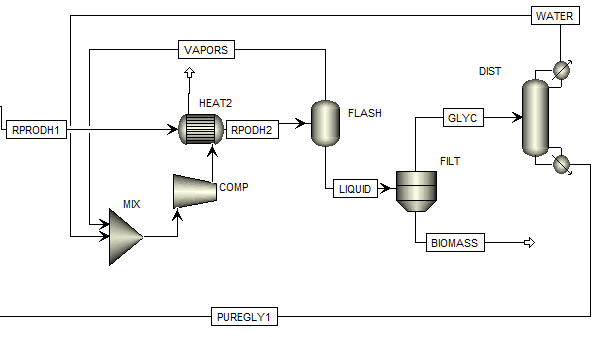
\includegraphics[width=.9\linewidth]{/home/vidianos/Documents/7o_εξάμηνο/Σχεδιασμός_Ι/Project/git_repo/Final_exam_files/Block_500_-_Καθαρισμός_Γλυκερόλης/2023-01-10_19-09-31_screenshot.png}
\caption{Διάγραμμα ροής του block 500}
\end{figure}

Στο block 500 γίνεται ο καθαρισμός του ρεύματος εξόδου του
βιοαντιδραστήρα παραγωγής γλυκερόλης. Αρχικά το ρεύμα προθερμαίνεται
και ύστερα εκτονώνεται σε έναν flash, στη συνέχεια εισέρχεται σε μία
φυγόκεντρο για την απομάκρυνση της στερέης φάσης, την βιομάζα, και τέλος
μια αποστακτική στήλη για τον τελικό καθαρισμό της γλυκερόλης.

\section{Σχεδιαστικές Επιλογές}
\label{sec:org8dd060e}
Το ρεύμα εξόδου προς καθαρισμό έχει 3 φάσεις, αέρια που είναι \(O_2\)
και \(CO_2\), στερεή που είναι βιομάζα, και υγρή που έχει νερό, οξικό
οξύ, γλυκερόλη, γλυκόζη, ουρία και αιθανόλη. Αρχικά επειδή το ρεύμα
έχει πολύ μεγάλη ποσότητα σε νερό, επιλέχθηκε ένας flash διαχωριστήρας,
εφόσον τα υγρά συστατικά έχουν χαμηλό σημείο βρασμού έως 120 \(^{o} C\)
πέρα από την γλυκερόλη που έχει σημείο βρασμού στους 290\(^{o} C\).
Παρακάτω παρουσιάζονται οι συνθήκες λειτουργίας στο flash.

\begin{table}[htbp]
\caption{Συνθήκες λειτουργίας του flash}
\centering
\begin{tabular}{ll}
Μέγεθος & Τιμή\\
\hline
Θερμοκρασία Εισόδου & 150 C\\
Θερμοκρασία Λειτουργίας & 140 C\\
Πίεση Λειτουργίας & 1 atm\\
\end{tabular}
\end{table}

Η πίεση παραμένει στη 1atm εφόσον δεν υπάρχει λόγος να αλλάξει εφόσον
υπάρχει μεγάλη διαφορά στα σημεία βρασμού μεταξύ του προιόντος και των
άλλων συστατικών. Η θερμοκρασία προθέρμανσης και λειτουργίας επιλέχθηκαν
έτσι ώστε να μην είναι αρκετά υψηλή για να υπάρξουν απώλειες σε
γλυκερόλη αλλά ούτε αρκετά χαμηλή που να παραμένει μεγάλη ποσότητα
νερού επειδή έτσι καθισταταί πιο ενεργοβόρα και κοστοβόρα η απόσταξη
αργότερα. Μετά απο διάφορες δοκιμές επιλέχθηκαν αυτές οι θερμοκρασίες
για τους παραπάνω λόγους.

Τέλος το ρεύμα καταλήγει σε μια αποστακτική στήλη για να απομακρυνθεί το
υπόλοιπο νερό ώστε να καθαριστεί πλήρως η γλυκερόλη, παράλληλα σε
αυτή την διεργασία απομακρύνεται όλη η εναπομένουσα αέρια φάση. Παρακάτω
παρουσιάζονται οι συνθήκες λειτουργίας στην αποστακτική στήλη τύπου
Radfrac.

\begin{table}[htbp]
\caption{Συνθήκες Λειτουργίας της Αποστακτικής}
\centering
\begin{tabular}{ll}
Μέγεθος & Τιμή\\
\hline
Θερμοκρασία εισόδου & 140 C\\
Θερμοκρασία λειτουργίας & 140 C\\
Πίεση κορυφής & 0.95 atm\\
Πίεση πυθμένα & 1.05 atm\\
Βαθμίδες & 6\\
Βαθμίδα Τροφοδοσίας & 3\\
Λόγος Αναρροής & 0.175\\
Λόγος αποστάγματος προς τροφοδοσία & 0.366\\
\end{tabular}
\end{table}

Η επιλογή των χαρακτηριστικών της στήλης έγιναν με βάση μια πρώτη
προσομοίωση με στήλη dstwu, ύστερα με βάση τα αποτελέσματά της έγινε
προσομοίωση σε radfrac. Η θερμοκρασία εισόδου και λειτουργίας δεν υπήρχε
λόγος να μεταβληθεί, όπως και η πίεση λειτουργίας λόγω της μεγάλης
διαφοράς στα σημεία βρασμού των υγρών συστατικών.

\subsection{Ενεργειακή Ολοκλήρωση}
\label{sec:orgfd1ea84}
Η προθέρμανση του ρεύματος επιτυγχάνεται εξ ολοκλήρου από τα θερμά
ρεύματα της διεργασίας. Αρχικά το καθαρό ρεύμα γλυκερόλης, εξέρχεται
από την στήλη στους 290\(^{o} C\) , το οποίο είναι ακατάλληλο για
αποθήκευση σε κάποια δεξαμενή, για αυτόν τον λόγο χρησιμοποιείται για
προθέρμανση του ρεύματος για την είσοδο στο flash, όμως λόγο της χαμηλής
θερμοχωρητικότητας της σε σχέση με αυτή του νερού δεν μεταβάλλει την θερμοκρασία. Συνεπώς πρέπει
να αξιοποιηθούν τα αέρια ρεύματα του flash και της αποστακτικής στήλης.
Όμως επειδή αυτά βρίσκονται σε πίεση 1 atm όπως και το ψυχρό ρεύμα, δεν
επιτυγχάνεται επαρκή θέρμανση, για αυτό αν γίνει συμπίεση του θερμού
ρεύματος στις 2atm, ολοκληρώνεται η προθέρμανση του ρεύματος.

\section{Υπολογισμοί}
\label{sec:org56f20c8}
Από τον βιοαντιδραστήρα παράγονται 13001 τόννοι γλυκερόλης τον
χρόνο, και από το τελικό ρεύμα ανακτούνται 11722 τόνοι, που αποτελεί το
90\%, δηλαδή χάνεται το 10\% της παραγόμενης γλυκερόλης στα αέρια
ρεύματα του flash και της αποστακτικής. Επίσης το τελικό ρεύμα
γλυκερόλης έχει καθαρότητα 99,99\%.

\section{Προσομοιώσεις στο Aspen}
\label{sec:org9f93df7}
Το μοντέλο που χρησιμοποιήθηκε για την προσομοίωση είναι το NRTL-HOC. Εφόσον το ρεύμα αυτό είναι συνέχεια του block 400, έχει τα ίδια συστατικά και άρα η αιτιολόγηση του μοντέλου είναι η ίδια. Το ρεύμα εισόδου της διεργασίας είναι στην ουσία τα προιόντα της βιοαντίδρασης όπως βγαίνουν από το block 400. Οδηγείται στους εναλλάκτες, οι οποίοι χρησιμοποιήθηκαν για την θέρμανση του και έπειτα μπαίνει στο flash.

Για τον διαχωρισμό της βιομάζας χρησιμοποιήθηκε ένα CFuge με το μοντέλο Decanter η οποία είναι η βασική διεργασία του Aspen για τον διαχωρισμό υγρού στερεού. Αυτό τοποθετήθηκε μετά το flash για να επιβεβαιωθεί ότι το μίγμα που τροφοδοτείται σε αυτόν δεν έχει αέρια φάση, όπως θα συνέβαινε αν ο decanter αυτός ήταν στην έξοδο του βιοαντιδραστήρα επειδή δεν υπάρχει πρότυπη μέθοδος για διαχωρισμό στερεού από μίγμα υγρού-ατμού.

Για την αποστακτική στήλη, αρχικά αυτή προσομοιώθηκε ως DSTWU ορίζοντας ελαφρύ (νερό) και βαρύ κλειδί (γλυκερόλη), ένα reflux ratio το οποίο δεν είναι ανάγκη να είναι σωστό σε πρώτη φάση, πτώση πίεσης στην στήλη και ορίζοντας την ανάκτηση στο απόσταγμα ώστε να έχει αρκετά μικρή ποσότητα γλυκερόλης (για να μην υπάρχουν απώλειες) και σχεδόν όλο το νερό. Από τα αποτελέσματα της στήλης αυτής βρέθηκαν οι σχεδιαστικές παραμέτροι που απαιτεί η στήλη Radfrac και προσομοιώθηκε με αυτά.
\end{document}